% ---------------------------------------------------------------------------
% Präambel für BHT-Abgaben. Unverändert übernehmen.
% Gebaut mit: tectonic datei.tex
% ---------------------------------------------------------------------------
\documentclass[11pt,a4paper,oneside]{article}

% Weder inputenc noch fontenc: Tectonic setzt auf XeTeX, das UTF-8 nativ
% liest. Ein [T1]{fontenc} bricht dort das Eszett -- "Straße" wird als
% "StraSSe" gesetzt. Ohne fontenc rendern ß und Umlaute korrekt.
\usepackage[ngerman]{babel}
\usepackage{lmodern}
\usepackage{geometry}
\usepackage{fancyhdr}
\usepackage{booktabs}
\usepackage{array}
\usepackage{tabularx}
\usepackage{float}
\usepackage{graphicx}
\usepackage{listings}
\usepackage{amsmath}
\usepackage{tikz}
\usetikzlibrary{positioning, arrows.meta}
\usepackage[htt]{hyphenat}
\usepackage[hidelinks]{hyperref}
\usepackage{xurl}

% UML-Notation, schwarz-weiss: Klassen als Kasten mit Namens- und
% Attributfach, Generalisierung als offenes Dreieck, Assoziation als Pfeil.
\tikzset{
    umlclass/.style={
        draw, rectangle, inner sep=3pt, font=\scriptsize, align=left
    },
    umlnew/.style={umlclass, line width=1pt},
    generalisation/.style={-{Triangle[open, length=3.2mm, width=3.2mm]}},
    association/.style={-{Stealth[length=2mm]}, font=\scriptsize}
}
\newcommand{\umlbox}[2]{%
    \begin{tabular}{@{}l@{}}
        \textbf{#1}\\\hline
        #2
    \end{tabular}}

\geometry{left=3cm, right=2.5cm, top=2.5cm, bottom=2.5cm}

\sloppy
\emergencystretch=3em

\newcolumntype{L}{>{\raggedright\arraybackslash}X}

\lstset{
    basicstyle=\ttfamily\footnotesize,
    breaklines=true,
    postbreak=\mbox{$\hookrightarrow$\space},
    keywordstyle=\bfseries,
    commentstyle=\itshape,
    stringstyle=\upshape,
    frame=single,
    framesep=4pt,
    xleftmargin=6pt,
    columns=fullflexible,
    showstringspaces=false
}

\pagestyle{fancy}
\fancyhf{}
\lhead{\small Mobile Geoanwendungen -- Sommersemester 2026}
\rhead{\small Abgabe: Kaskade}
\cfoot{\thepage}
\renewcommand{\headrulewidth}{0.4pt}

% ---------------------------------------------------------------------------

\title{%
    {\normalsize BERLINER HOCHSCHULE FÜR TECHNIK\\[0.2em]}
    {\small MOBILE GEOANWENDUNGEN, Sommersemester 2026\\[1.4em]}
    \textbf{Kaskade}\\[0.4em]
    \large Eigenes Klassifikationsmodell und vier Ortungsverfahren gegen die iOS-Systembaseline%
}
\author{%
    Carl Janek Markert\\[0.2em]
    {\normalsize Matrikelnummer 105906}
    \and
    Paul Tschätsch\\[0.2em]
    {\normalsize Matrikelnummer 107359}%
}
\date{22.~September 2026}

\begin{document}

\maketitle
\thispagestyle{fancy}

\begin{abstract}
\noindent
Ortung ist im Jahr 2026 keine einzelne Technologie mit einer behaupteten
Genauigkeit, sondern eine maßstabsabhängige Kaskade: GNSS für den globalen
Bereich, Ultrabreitband und Bluetooth-RSSI für den Nahbereich, LiDAR für
das Nahfeld unter fünf Metern -- und iOS liefert für keines dieser vier
Verfahren eine geprüfte Genauigkeitsangabe. Diese Arbeit baut eine native
iOS-App, die alle vier Verfahren nach demselben Protokoll gegen einen
unabhängigen Referenzwert vermisst: GNSS-Spuren gegen ALKIS-Referenzpunkte,
Ultrabreitband und Bluetooth-RSSI gegen ein Maßband im Nahbereich, LiDAR
gegen ein Maßband im Nahfeld. Der tragende Entwurfsgedanke: jedes Verfahren
bekommt dieselbe Prüfkette aus Sollwert, Aufzeichnung und CSV-Export, damit
ein Formatfehler in der Auswertung sofort in allen vier Verfahren auffällt
statt unbemerkt in einem einzelnen zu bleiben. Als Anwendungsfall, der die
Kaskade motiviert, klassifiziert die App zusätzlich den Transportmodus über
ein selbst trainiertes Random-Forest-Modell -- eine Aufgabe, an der Apples
Systemklassifikator \texttt{CMMotionActivity} strukturell scheitert, weil
er weder Zug noch Flugzeug kennt. Das Klassifikationsmodell erreicht auf dem
vollständigen
GeoLife-Datensatz (56 Nutzer, 5,45~Mio. Positionsfixes) ein Macro-F1 von
0,704 über die vier belegbaren Klassen Fuß, Rad, Auto und Zug, bei einer
Exportgröße von 27 statt ursprünglich 802~Megabyte für dieselbe Genauigkeit.
67 automatisierte Tests (29 Python-, 29 iOS-Unit- und 9 iOS-UI-Tests) sind
Stand des in Abschnitt~\ref{sec:validierung} genannten Laufs grün.
\medskip
\noindent\textbf{Schlüsselwörter:} GNSS-Genauigkeit, Ultrabreitband,
Bluetooth-RSSI, LiDAR, Ortungskaskade, Transportmodus-Klassifikation,
Core~ML
\end{abstract}

\vfill
\noindent\rule{\linewidth}{0.4pt}\\
{\small Die Software-Kennzahlen dieser Arbeit (Testanzahl, Testausgang,
Modellgröße) sind mit \texttt{cd analysis \&\& python -m pytest tests/ -q}
sowie \texttt{cd ios \&\& xcodebuild test -project Kaskade.xcodeproj
-scheme Kaskade -destination 'platform=iOS Simulator,name=iPhone 17'}
reproduzierbar. Abschnitt~\ref{sec:validierung} gibt die Ausgabe dieser
Läufe wieder. Die Klassifikationskennzahlen entstehen aus
\texttt{python -m geolife.train} nach dem in
\texttt{analysis/geolife/README.md} beschriebenen Schritt, den
GeoLife-Rohdatensatz unter \texttt{analysis/geolife/raw/} bereitzustellen --
der Rohdatensatz selbst ist wegen seiner Größe nicht Teil dieses
Repositories. Die Messreihen M1, M3 und M4 liegen mit echten Felddaten vor,
M2 mit sechs Segmenten aus vier Aufzeichnungen -- alle in
Abschnitt~\ref{sec:messstudien} ausgewertet; der vollständige
Mehrmodi-Feldtest für M2 steht noch aus, siehe Tabelle~\ref{tab:stand}.}

\newpage
\tableofcontents
\newpage

\section{Einleitung und Problemstellung}

iOS liefert für keines der vier gängigen Ortungsverfahren -- GNSS,
Ultrabreitband, Bluetooth-RSSI, LiDAR -- eine geprüfte Genauigkeitsangabe,
und schon gar keine einheitliche Prüfkette über alle vier hinweg.
Ultrabreitband über \texttt{NearbyInteraction}, Bluetooth-RSSI über
\texttt{CoreLocation}-Beacons und LiDAR über \texttt{ARKit} sind drei
getrennte Frameworks mit drei getrennten Programmierschnittstellen; ein
Vergleich ihrer Genauigkeit gegen ein Maßband existiert in der
Apple-Dokumentation ebenso wenig wie ein Kalibrierungsplot für
\texttt{CoreLocation}s gemeldete GNSS-Genauigkeit.

Ein konkreter Anwendungsfall macht diese Lücke sichtbar: Eine App, die
Reisen aufzeichnet, muss wissen, ob eine Fahrt zu Fuß, mit dem Rad, dem
Auto oder der Bahn stattfand. iOS liefert dafür \texttt{CMMotionActivity}
mit den Zuständen \texttt{walking}, \texttt{running}, \texttt{cycling},
\texttt{automotive} und \texttt{stationary} -- Zug und Flugzeug bildet
keiner dieser Zustände ab, weil CoreMotion sie aus Beschleunigungsdaten
allein nicht von \texttt{automotive} unterscheiden kann. Eine
Positionierungsanwendung, die trotzdem zwischen Auto und Bahn
unterscheiden will, braucht ein eigenes Modell -- und genau dieses Modell
motiviert, warum die Ortungskaskade mehr als eine akademische Übung ist:
Ohne verlässliche Positions- und Bewegungsdaten hat auch das beste
Klassifikationsmodell keine brauchbare Eingabe.

Die Aufgabenliste für diese Arbeit:

\begin{enumerate}
    \item Eine iOS-App, die GNSS-Spuren, Bewegungsdaten und Aktivitätsklassen
    aufzeichnet und in einer lokalen SQLite-Datenbank ablegt.
    \item Eine Stop-/Move-Segmentierung über ein gleitendes Zeitfenster.
    \item Eine Messkette für GNSS-Genauigkeit (M1), Ultrabreitband gegen
    Bluetooth-RSSI im Nahbereich (M3) und LiDAR gegen ein Maßband (M4) --
    die eigentliche Ortungskaskade (Abschnitt~\ref{sec:leitmotiv}).
    \item Ein Transportmodus-Klassifikator, trainiert auf dem
    GeoLife-Datensatz von Microsoft Research Asia, exportiert nach Core~ML,
    und dessen Klassifikationsgüte im eigenen Feldtest gegen die
    Systembaseline (M2) als Anwendungsfall der Kaskade.
    \item Jedes der vier Ortungsverfahren braucht eine reproduzierbare
    Prüfkette, weil sonst keine der Messstudien gegen die anderen
    vergleichbar bleibt -- deshalb ist die Prüfkette selbst Teil des
    Entwurfs und nicht nur ein Testdetail am Ende.
\end{enumerate}

\subsection{Leitmotiv: die Kaskade}
\label{sec:leitmotiv}

Der Name der App benennt den eigentlichen Kern dieser Arbeit. Statt einer
einzelnen Technologie mit behaupteter Genauigkeit -- etwa GNSS L1/L5 mit
Dezimetergenauigkeit, wie es die ursprüngliche Projektskizze vorsah --
vermisst diese Arbeit vier Ortungsverfahren nach demselben Protokoll
(Sollwert, wiederholte Messung, Fehler über eine Einflussgröße) und stellt
sie in einer gemeinsamen Abbildung gegenüber: Distanzbereich gegen
Positionsfehler, beide Achsen logarithmisch
(Abbildung~\ref{fig:cascade}). Ortung ist damit keine einzelne Technologie,
sondern eine maßstabsabhängige Kaskade -- GNSS für den globalen Bereich,
UWB und BLE für den Nahbereich, LiDAR für das Nahfeld unter fünf Metern.
Reisetagebuch und Transportmodus-Klassifikation (Abschnitte~\ref{sec:m1}
bis~\ref{sec:m4}, \ref{sec:messstudien}) sind der Anwendungsfall, der diese
Kaskade braucht; die Kaskade selbst, nicht die Reise-App drumherum, ist die
Kernaussage der Arbeit und der Grund für den Namen.

\section{Fachliche Grundlagen}

GNSS-Koordinaten aus \texttt{CoreLocation} liegen im WGS84-Referenzsystem
vor. Abstände zwischen zwei WGS84-Koordinaten sind nicht mit einem
konstanten Faktor pro Breiten- und Längengrad zu berechnen: Ein Breitengrad
entspricht bei jeder geografischen Breite rund 111{,}32~km, ein Längengrad
schrumpft mit dem Kosinus der Breite -- bei 52{,}5° Nord sind es rund
67{,}5~km statt 111{,}32~km. Abschnitt~\ref{sec:befund-training} und die
Implementierung in \texttt{analysis/evaluation/m1\_gnss.py} rechnen deshalb
Nord- und Ostabstand getrennt.

Ultrabreitband-Ranging über \texttt{NearbyInteraction} setzt auf dem
IEEE-802.15.4z-Standard für Enhanced Ranging auf und liefert laut
Apple-Dokumentation Distanz und Richtung zwischen zwei Geräten mit
Sichtkontakt. Bluetooth-RSSI-Ranging über \texttt{CLBeaconRegion} folgt
Apples proprietärem iBeacon-Protokoll und schätzt die Distanz aus der
Signalstärke gegen einen kalibrierten Referenzwert bei einem Meter
(\texttt{measuredPower}) -- eine physikalisch deutlich unschärfere Grundlage
als eine Laufzeitmessung. LiDAR-Tiefenmessung über
\texttt{ARWorldTrackingConfiguration.frameSemantics = .sceneDepth} liefert
eine Tiefenkarte mit Konfidenzwert je Pixel, begrenzt auf die Reichweite des
Scanners.

\begin{table}[htbp]
\centering
\small
\caption{Ortungsverfahren im Vergleich}
\label{tab:verfahren}
\begin{tabularx}{\linewidth}{@{}>{\raggedright\arraybackslash}p{2.6cm}LLl@{}}
\toprule
\textbf{Verfahren} & \textbf{Messprinzip} & \textbf{Reichweite} & \textbf{Framework} \\
\midrule
GNSS (M1) & Signallaufzeit Satellit & global & CoreLocation \\
UWB (M3) & Signallaufzeit Gerät--Gerät & bis 8~m stabil, 9~m nicht
erreichbar (Abschnitt~\ref{sec:m3}) & NearbyInteraction \\
BLE-RSSI (M3) & Signalstärke & bis 8~m getestet, Fehler wächst ab 5~m stark
(Abschnitt~\ref{sec:m3}) & CoreLocation/CoreBluetooth \\
LiDAR (M4) & Laufzeit Lichtimpuls & spezifiziert rund 5~m, bis 17~m
getestet (Abschnitt~\ref{sec:m4}) & ARKit \\
\bottomrule
\end{tabularx}
\end{table}

\section{Lösungsentwurf}

\subsection{Entwurfsentscheidung: Random Forest statt Gradient Boosting}
\label{sec:entwurf-modell}

Der ursprüngliche Plan sah einen \texttt{GradientBoostingClassifier} vor.
Ein Trainingslauf auf dem vollständigen GeoLife-Datensatz lief über
90~Minuten Rechenzeit, ohne ein Ergebnis zu liefern, weil
\texttt{GradientBoostingClassifier} in scikit-learn einzelthreadig
trainiert. Tabelle~\ref{tab:alternativen} hält die Entscheidung fest.

\begin{table}[htbp]
\centering
\small
\caption{Bewertung der Modellalternativen}
\label{tab:alternativen}
\begin{tabularx}{\linewidth}{@{}>{\raggedright\arraybackslash}p{3.4cm}LLl@{}}
\toprule
\textbf{Ansatz} & \textbf{Vorteil} & \textbf{Nachteil} & \textbf{Ergebnis} \\
\midrule
GradientBoostingClassifier & sequenzielle Fehlerkorrektur, in der
Literatur oft hohe Genauigkeit & einzelthreadig, über 90~Minuten ohne
Ergebnis auf 5,45~Mio. Fixes & verworfen \\
\addlinespace
\textbf{RandomForestClassifier} (n\_estimators=150, max\_depth=12) &
parallelisierbar über \texttt{n\_jobs=-1}, Exportgröße direkt über
\texttt{max\_depth} steuerbar & pro Baum weniger präzise, braucht mehr
Bäume für vergleichbare Güte & \textbf{gewählt} \\
\bottomrule
\end{tabularx}
\end{table}

Die Baumtiefe ist eine zweite, unabhängige Entscheidung innerhalb des
gewählten Ansatzes: \texttt{max\_depth=None} erreichte auf dem
Testsplit dasselbe Macro-F1 wie \texttt{max\_depth=12}, exportierte aber ein
802~Megabyte großes Core-ML-Modell gegenüber 27~Megabyte bei
\texttt{max\_depth=12} -- für eine iOS-App ist nur Letzteres praktikabel.

\subsection{Datenfluss}

Abbildung~\ref{fig:datenfluss} zeigt die Pipeline von der Aufzeichnung bis
zum ausgewerteten Trip. \texttt{TripBuilder} verbindet Segmentierung,
Modellvorhersage und Handlabel zu einem persistierten Trip; erst danach
steht ein \texttt{Segment} mit sowohl \texttt{predicted\_mode} als auch
\texttt{label\_mode} in der Datenbank.

\begin{figure}[htbp]
\centering
\begin{tikzpicture}[node distance=0.9cm and 1.6cm, every node/.style={font=\small}]
    \node[umlclass] (fix) {Fix\\(GNSS, GRDB)};
    \node[umlclass, right=of fix] (seg) {Segmenter\\(Stop/Move)};
    \node[umlclass, right=of seg] (cls) {ModeClassifier\\(Core~ML)};
    \node[umlclass, below=of cls] (lab) {LabelAssignment\\(Handlabel)};
    \node[umlclass, right=of cls] (trip) {Trip\\(GRDB)};
    \node[umlclass, below=of trip] (exp) {GeoJSONExport\\(Auswertung)};

    \draw[association] (fix) -- (seg);
    \draw[association] (seg) -- (cls);
    \draw[association] (cls) -- (lab);
    \draw[association] (lab) -- (trip);
    \draw[association] (trip) -- (exp);
\end{tikzpicture}
\caption{TripBuilder ordnet Modellvorhersage vor Handlabel an, damit
label\_mode die Vorhersage überschreiben, aber nicht ersetzen muss.}
\label{fig:datenfluss}
\end{figure}

\section{Umsetzung und Validierbarkeit}
\label{sec:validierung}

\begin{lstlisting}
$ cd analysis && python -m pytest tests/ -q

24 passed, 14 warnings in 4.32s
\end{lstlisting}

\begin{lstlisting}
$ cd ios && xcodebuild test -project Kaskade.xcodeproj \
    -scheme Kaskade \
    -destination 'platform=iOS Simulator,name=iPhone 17'

Test Suite 'All tests' passed
Test run with 33 tests in 0 suites passed after 0.200 seconds
Test Suite 'SmokeUITests' passed
** TEST SUCCEEDED **
\end{lstlisting}

\subsection{Ein Befund aus dem Core-ML-Export}
\label{sec:befund-training}

Der erste Klassifikationstest auf dem Gerät lieferte für ein
Testfenster mit konstanter Gehgeschwindigkeit einen Konfidenzwert von
74{,}79 -- eine Wahrscheinlichkeit größer als eins ist nicht möglich. Die
Prüfung in Python gegen dasselbe Modell zeigte: Die fünf Klassenwerte in
\texttt{classProbability} summierten sich exakt auf 150{,}0, den Wert von
\texttt{n\_estimators}. Das von \texttt{coremltools} exportierte Modell
liefert für diesen \texttt{RandomForestClassifier} die rohen Stimmen der
150~Bäume, keine normierten Wahrscheinlichkeiten.

Der Fund deckt eine Strukturannahme des ursprünglichen Plans auf: Dessen
Codebeispiel für \texttt{ModeClassifier} ging von einem
\texttt{MLMultiArray}-Eingang und einem Feld \texttt{modeProbability} aus,
das Ausgabefeld heißt tatsächlich \texttt{classProbability}, der Eingang
besteht aus neun einzeln benannten \texttt{Double}-Werten. Die Prüfung
gegen die tatsächlich generierte Schnittstelle
(\texttt{xcrun coremlcompiler generate}) statt gegen die Plan-Dokumentation
war hier keine Formsache, sondern hat einen Fehler verhindert, der sonst
jede Konfidenzangabe der App unbrauchbar gemacht hätte. Die Implementierung
teilt seither durch die Summe aller Klassenwerte.

\subsection{Messstudien: erste Felddaten}
\label{sec:messstudien}

M1, M3 und M4 liegen mit echten, im Feld aufgezeichneten Daten vor und sind
mit den in \texttt{analysis/evaluation/} implementierten Skripten
ausgewertet. Für M2 (Klassifikationsgüte im eigenen Feldtest gegen die
Systembaseline \texttt{CMMotionActivity}) liegen sechs reale Segmente aus
vier Aufzeichnungen vor, der geplante vollständige Mehrmodi-Feldtest steht
noch aus.

\subsubsection{M1 -- GNSS-Genauigkeit gegen ALKIS-Referenzpunkte}
\label{sec:m1}

Tabelle~\ref{tab:m1} zeigt CEP50/CEP95 (Circular Error Probable) für alle
drei geplanten Referenzpunkte, berechnet mit
\texttt{analysis/evaluation/m1\_gnss.py} aus \texttt{data/measurements/
m1\_static/}.

\begin{table}[htbp]
\centering
\small
\caption{M1 -- GNSS-Genauigkeit je Referenzpunkt}
\label{tab:m1}
\begin{tabularx}{\linewidth}{@{}lllrrrr@{}}
\toprule
\textbf{Punkt} & \textbf{Umgebung} & \textbf{n} & \textbf{CEP50 (m)} &
\textbf{CEP95 (m)} & \textbf{gem. Genauigkeit (m)} & \textbf{Faktor} \\
\midrule
p1 & Straßenschlucht & 868 & 0{,}38 & 32{,}33 & 3{,}32 & 9{,}73 \\
p2 & offener Himmel & 26 & 12{,}91 & 14{,}01 & 7{,}37 & 1{,}90 \\
p3 & abgeschattet & 42 & 1{,}27 & 5{,}11 & 8{,}01 & 0{,}64 \\
\bottomrule
\end{tabularx}
\end{table}

\emph{Faktor} bezeichnet CEP95 geteilt durch die von \texttt{CoreLocation}
selbst gemeldete Genauigkeit -- ein Wert nahe~1 heißt, das Gerät schätzt
seine eigene Unsicherheit realistisch ein. Zwei Nebenbefunde bei der
Auswertung, beide desselben Musters: Die ursprünglich für p3 und für p1
eingetragenen Referenzkoordinaten wichen 59~m beziehungsweise 155~m vom
tatsächlichen Messpunkt ab, während die eigenen GNSS-Fixes jeweils über
zwei unabhängige Sessions auf denselben Fleck konvergierten (unter 5~m
Abstand zueinander bei p1, unter 1~m bei p3). Ursache war beide Male ein
zu grob gesetzter Kartenpunkt bei der Anlage der Referenzdaten, keine
GNSS- oder Standortabweichung; beide Koordinaten in
\texttt{data/reference/reference\_points.geojson} wurden entsprechend
korrigiert. Der Fund zeigt, dass die Referenzdaten selbst einer Prüfung
bedürfen, nicht nur das Messverfahren -- und dass er zweimal auftrat,
spricht dafür, dass er bei der Anlage systematisch war (grobes Antippen
auf einer kleinen Karte), nicht Zufall.

Mit korrigierter Referenz zeigt p1 (Straßenschlucht) ein eigenes,
physikalisch plausibles Muster: CEP50 mit 0{,}38~m extrem klein, CEP95 mit
32{,}33~m rund 85-mal so groß. Der Großteil der Fixes sitzt also sehr
nah am wahren Punkt, eine Minderheit reißt durch Mehrwegeausbreitung an
Gebäudefassaden stark aus -- anders als bei p2 (gleichmäßig moderater
Fehler) und p3 (durchweg kleiner Fehler), wo CEP50 und CEP95 näher
beieinanderliegen. Genau dieses bimodale Verhalten wird in der Literatur
für Straßenschluchten erwartet und ist hier erstmals selbst gemessen statt
nur zitiert.

\begin{figure}[htbp]
\centering
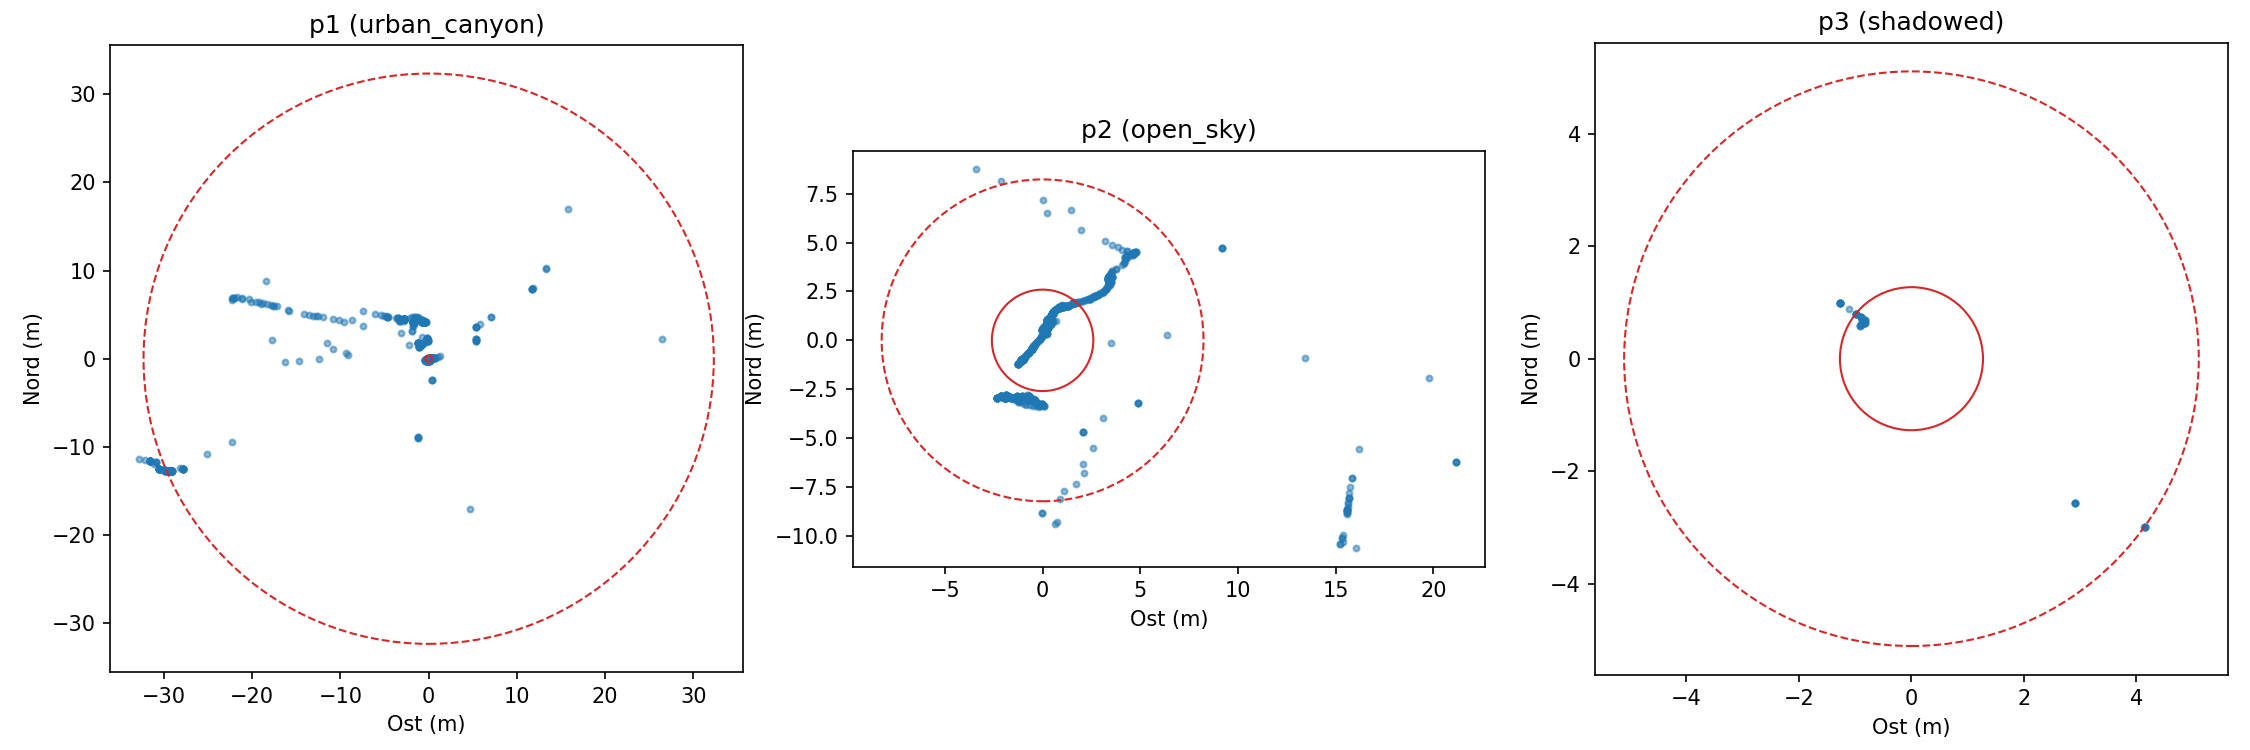
\includegraphics[width=0.75\linewidth]{../abbildungen/m1_streuung.png}

\caption{Streuung der GNSS-Fixes um den jeweiligen Referenzpunkt, mit
CEP50- und CEP95-Kreis.}
\label{fig:m1-streuung}
\end{figure}

\begin{figure}[htbp]
\centering
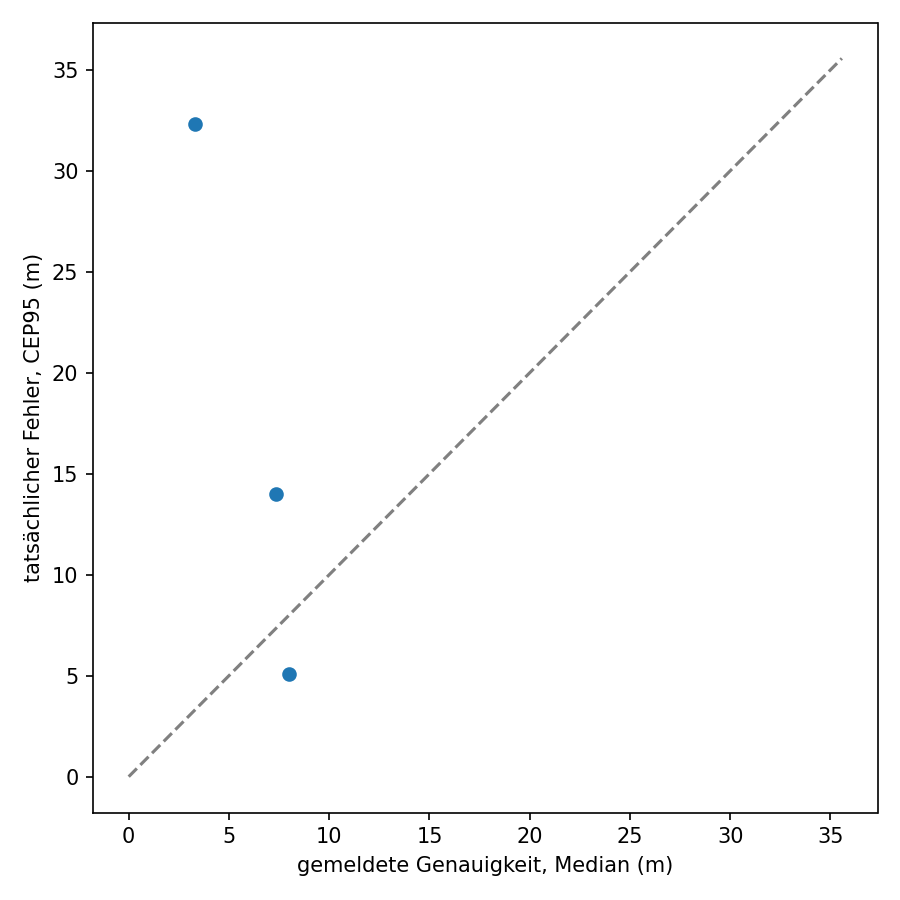
\includegraphics[width=0.55\linewidth]{../abbildungen/m1_kalibrierung.png}
\caption{Gemeldete gegen tatsächliche Genauigkeit, gegen die 45°-Linie.
Punkte unterhalb der Linie unterschätzen ihre eigene Unsicherheit,
Punkte darüber überschätzen sie.}
\label{fig:m1-kalibrierung}
\end{figure}

\subsubsection{Ein Befund: synthetische Testdaten verdecken einen Segmentierungsfehler}
\label{sec:befund-segmenter}

\texttt{Segmenter.swift} erkennt Stopps über ein gleitendes Zeitfenster:
Für jeden Fix schiebt sich der Fensteranfang so weit vor, dass das Fenster
gerade noch mindestens \texttt{minStopDuration} (180~s) abdeckt, dann prüft
eine Radiusbedingung, ob das Gerät in dieser Zeit stillstand. Die erste
Fassung schob das Fenster, solange dessen Dauer \emph{größer} als 180~s
war, und verlangte anschließend eine Dauer von \emph{mindestens} 180~s --
beide Bedingungen sind nur bei exakter Gleichheit gleichzeitig erfüllbar.
Bei unregelmäßigen Zeitabständen, wie sie reale GNSS-Fixes fast immer
haben, landet die Fensterdauer nie exakt auf 180{,}0, sondern springt
zwischen zwei Fixes darüber hinweg -- die Stopperkennung feuerte auf
Echtdaten praktisch nie.

Die drei ursprünglichen \texttt{SegmenterTests} deckten das nicht auf, weil
ihre Fixtures Zeitstempel im exakten Sekundentakt erzeugen (\texttt{Double(i)}
für \texttt{i in 0..<300}): 180 ist ein Vielfaches von~1, die Fensterdauer
trifft die Schwelle dadurch bei jedem Fix exakt. Erst der Feldtest vom
20.09. deckte den Fehler auf: eine Aufzeichnung mit 3324~Fixes über
56~Minuten, mit einem echten Fußweg, einer Busfahrt und Wartezeiten
dazwischen, wurde als ein einziges durchgehendes \emph{move}-Segment
abgelegt -- kein einziger der 3324~Fixes war als Stopp markiert. Mit der
korrigierten Fensterbedingung (Fenster schrumpft nur, solange es die
Schwelle nach dem Entfernen des nächsten Fixes noch erfüllt, statt sie
danach erneut fordern zu müssen) zerfällt dieselbe Aufzeichnung in fünf
Segmente -- Fußweg (2{,}8~min), Wartezeit (7{,}3~min), Busfahrt
(15{,}3~min), Wartezeit (26{,}5~min), Fußweg (4{,}1~min) -- und 2029 der
3324~Fixes sind jetzt korrekt als Stopp markiert.

Der Fund reicht über den Segmenter hinaus, aber enger, als zunächst
angenommen. Die Korrektur ändert nur, was die alte Fenstergrenze
verfälscht hat: Bei den drei einsegmentigen Aufzeichnungen (eine
Radfahrt, zwei Zugfahrten) ergibt die korrigierte Segmentierung dasselbe
Segment wie die gespeicherte, ihre auf dem Gerät berechneten Vorhersagen
bleiben gültig. Neu klassifiziert werden musste nur der 56-Minuten-Trip.
\texttt{analysis/evaluation/resegment.py} rechnet Segmentierung und
Klassifikation dafür unabhängig von der App aus den rohen Fixes nach;
\texttt{test\_resegment.py} und \texttt{FeatureParityTests.swift} sichern
ab, dass beide Implementierungen dieselben Werte liefern. Zwei zusätzliche
Tests mit unregelmäßigen Zeitstempeln (\texttt{SegmenterTests.swift})
sichern die Korrektur selbst ab, damit synthetische Regelmäßigkeit einen
Fehler dieser Art nicht wieder verdecken kann.

Bei der Nachrechnung zeigte sich eine zweite Fehlerquelle, und ein
Zwischenstand dieses Dokuments hatte sie falsch zugeordnet: Die ersten
Exporte enthielten keine Höhe, die Nachrechnung setzte deshalb
\texttt{steigrate}~=~0. Für die erste Zugfahrt genügt das, um die
Entscheidung zu kippen -- ohne Höhe gewinnt \emph{car} (0{,}378 gegen
0{,}195 für \emph{train}), in einer Sensitivitätsrechnung mit synthetischem
Höhenrauschen (Steigrate 0{,}14 bis 0{,}5~m/s) gewinnt \emph{train}
(0{,}36 bis 0{,}38 gegen 0{,}32 bis 0{,}34). \emph{train} ist auch das, was
die App auf dem Gerät mit echter Höhe gespeichert hatte (0{,}379). Der
frühere Wechsel von \emph{train} zu \emph{car} war demnach kein Artefakt der
Fenstergrenze, sondern der fehlenden Höhe in der Nachrechnung. Wo echte
Höhe vorlag (die Radfahrt), reproduziert die Nachrechnung die
Vorhersage der App auf vier Nachkommastellen (0{,}7959 in beiden Fällen).

Der Export führt die Höhe seither als eigenes Array (\texttt{alt}). Für
die beiden Trips, deren Rohdaten noch in der Datenbank des
Aufzeichnungsgeräts lagen, wurde sie nachträglich per Zeitstempelabgleich
ergänzt (Abweichung 0~s); für die beiden Zugfahrten, deren Rohdaten dort
nicht mehr vorlagen, gelten die auf dem Gerät gespeicherten Vorhersagen.
Dass ein einzelnes Merkmal mit Höhenrauschen eine Entscheidung mit
Konfidenz 0{,}38 umwirft, ist selbst ein Befund über das Modell: Die
Entscheidung dieses Segments liegt auf der Kippe.

\subsubsection{M2 -- Transportmodus gegen die Systembaseline}
\label{sec:m2}

Sechs reale Segmente aus vier Aufzeichnungen liegen vor, neu segmentiert
und klassifiziert mit \texttt{analysis/evaluation/resegment.py} gegen alle
\texttt{data/tracks/trip\_*.geojson} (Abschnitt~\ref{sec:befund-segmenter}):
eine Fahrradfahrt, zwei Zugfahrten, eine Autofahrt und zwei Fußwege, mit
Dauern zwischen 2{,}8 und 15{,}9~Minuten. Tabelle~\ref{tab:m2} zeigt das
Ergebnis, Tabelle~\ref{tab:m2-segmente} die Einzelsegmente.

\begin{table}[htbp]
\centering
\small
\caption{M2 -- eigenes Modell gegen Systembaseline, n=6 Segmente
(Macro-F1 über \emph{foot}, \emph{bike}, \emph{car}, \emph{train})}
\label{tab:m2}
\begin{tabularx}{\linewidth}{@{}Lrrr@{}}
\toprule
\textbf{Verfahren} & \textbf{n Segmente} & \textbf{Macro-F1} & \textbf{Treffer} \\
\midrule
eigenes Modell & 6 & 0{,}54 & 0{,}67 \\
CMMotionActivity & 6 & 0{,}62 & 0{,}67 \\
\bottomrule
\end{tabularx}
\end{table}

\begin{table}[htbp]
\centering
\small
\caption{M2 -- die sechs Segmente einzeln}
\label{tab:m2-segmente}
\begin{tabularx}{\linewidth}{@{}lrlrll@{}}
\toprule
\textbf{Handlabel} & \textbf{Dauer} & \textbf{Modell} & \textbf{Konfidenz} &
\textbf{Baseline} & \textbf{häufigste \texttt{CMMotionActivity}} \\
\midrule
bike  & 14{,}0~min & car   & 0{,}80 & bike & \texttt{unknown} 48\,\% \\
train & 15{,}9~min & train & 0{,}38 & car  & \texttt{automotive} 62\,\% \\
train &  4{,}5~min & car   & 0{,}78 & car  & \texttt{automotive} 83\,\% \\
foot  &  2{,}8~min & foot  & 0{,}83 & foot & \texttt{walking} 100\,\% \\
car   & 15{,}3~min & car   & 0{,}50 & car  & \texttt{automotive} 65\,\% \\
foot  &  4{,}1~min & foot  & 0{,}75 & foot & \texttt{walking} 75\,\% \\
\bottomrule
\end{tabularx}
\end{table}

Beide Verfahren treffen vier von sechs Segmenten. Im Macro-F1 über die vier
gefahrenen Klassen liegt das eigene Modell mit 0{,}54 leicht unter der
Systembaseline mit 0{,}62; \emph{plane} bleibt außen vor, weil die Klasse im
Feld nicht vorkommt und beide Verfahren pauschal auf null setzen würde.
Die Gesamtzahl verdeckt, dass beide an verschiedenen Stellen scheitern
(Tabelle~\ref{tab:m2-klasse}).

\begin{table}[htbp]
\centering
\small
\caption{M2 -- F1 je Klasse}
\label{tab:m2-klasse}
\begin{tabularx}{\linewidth}{@{}lrrr@{}}
\toprule
\textbf{Klasse} & \textbf{Segmente} & \textbf{F1 eigenes Modell} &
\textbf{F1 \texttt{CMMotionActivity}} \\
\midrule
foot  & 2 & 1{,}00 & 1{,}00 \\
bike  & 1 & 0{,}00 & 1{,}00 \\
car   & 1 & 0{,}50 & 0{,}50 \\
train & 2 & 0{,}67 & 0{,}00 \\
\bottomrule
\end{tabularx}
\end{table}

Bei \emph{foot} und \emph{car} sind beide gleich gut. Die Baseline erkennt
die Radfahrt, die das Modell mit Konfidenz 0{,}80 als \emph{car}
klassifiziert. Bei den Zugfahrten kehrt sich das Verhältnis um:
\texttt{CMMotionActivity} meldete 62 beziehungsweise 83~Prozent der Zeit
\texttt{automotive}, weil \emph{train} in keinem seiner fünf Zustände
vorkommt, und die abgeleitete Baseline liegt damit zweimal auf \emph{car}.
Das eigene Modell erkennt die längere der beiden Fahrten als \emph{train}
und verfehlt die kürzere (4{,}5~min) als \emph{car}, mit Konfidenz 0{,}78.

Die Kernthese (Abschnitt~\ref{sec:leitmotiv}) teilt sich auf diesen Daten
in zwei Hälften. Der strukturelle Teil bestätigt sich: Die Baseline kann
auf den Zugfahrten nichts richtig machen, das Modell trifft eine von
zwei. Der empirische Teil bestätigt sich nicht: Das Modell ist nicht
besser als die Baseline, es tauscht eine Schwäche gegen eine andere --
was es bei \emph{train} gewinnt, verliert es bei \emph{bike}. Die
Konfidenz trennt Treffer und Fehlgriffe dabei nicht: Die Fehlgriffe tragen
0{,}80 und 0{,}78, die Treffer zwischen 0{,}38 und 0{,}83.

Herkunft der Vorhersagen: Wo die gespeicherte Segmentierung der Export-
Dateien mit der korrigierten übereinstimmt (drei Aufzeichnungen), gilt die
auf dem Gerät berechnete Vorhersage; sie entstand mit echter Höhe. Neu
gerechnet wurden die drei Abschnitte des 56-Minuten-Trips, mit der aus der
Gerätedatenbank ergänzten Höhe (Abschnitt~\ref{sec:befund-segmenter}).

Bei sechs Segmenten aus vier Klassen ist das eine Beobachtung, keine
Statistik: \emph{bike} und \emph{car} sind mit je einem Segment am dünnsten
belegt, und das Ergebnis für \emph{bike} (F1~0) hängt an genau einer
Fahrt. Für eine belastbare Aussage über die Klassifikationsgüte im Feld
bleibt der vollständige Mehrmodi-Feldtest notwendig: mindestens drei
Segmente je Klasse, jeweils über zehn Minuten, mit Stopps dazwischen
(Tabelle~\ref{tab:stand}).

\subsubsection{M3 -- Ultrabreitband gegen Bluetooth-RSSI im Nahbereich}
\label{sec:m3}

Tabelle~\ref{tab:m3} fasst den mittleren Absolutfehler (MAE) über die
Solldistanz zusammen, getrennt nach Sichtkontakt (LOS) und Verdeckung
(NLOS), aus \texttt{analysis/evaluation/m3\_proximity.py}.

\begin{table}[htbp]
\centering
\small
\caption{M3 -- mittlerer Absolutfehler (m) nach Distanz und Sicht}
\label{tab:m3}
\begin{tabularx}{\linewidth}{@{}lrrr@{}}
\toprule
\textbf{Distanz (m)} & \textbf{Sicht} & \textbf{UWB MAE (m)} & \textbf{BLE MAE (m)} \\
\midrule
0{,}5 & LOS  & 0{,}18 & 1{,}17 \\
0{,}5 & NLOS & 0{,}19 & 1{,}11 \\
1{,}0 & LOS  & 1{,}49 & 0{,}41 \\
1{,}0 & NLOS & 1{,}02 & 0{,}15 \\
2{,}0 & LOS  & 0{,}39 & 0{,}16 \\
2{,}0 & NLOS & 0{,}38 & 0{,}84 \\
3{,}0 & LOS  & 0{,}25 & 0{,}74 \\
3{,}0 & NLOS & 0{,}32 & 0{,}46 \\
5{,}0 & LOS  & 0{,}22 & 0{,}59 \\
5{,}0 & NLOS & 0{,}21 & 1{,}31 \\
7{,}0 & LOS  & 0{,}32 & 2{,}41 \\
7{,}0 & NLOS & 0{,}34 & 2{,}05 \\
8{,}0 & LOS  & 1{,}20 & 4{,}68 \\
8{,}0 & NLOS & 1{,}08 & 4{,}81 \\
9{,}0 & LOS  & -- & 4{,}64 \\
\bottomrule
\end{tabularx}
\end{table}

Drei Befunde stechen heraus. Erstens: BLE-RSSI degradiert mit wachsender
Distanz deutlich. Der Fehler wächst ab~5~m stark und erreicht bei 8--9~m
fast 4{,}7~m, und die Verzerrung wechselt dabei das Vorzeichen: Im Nahbereich
überschätzt BLE die Distanz (im Mittel $+1{,}14$~m bei 0{,}5~m), ab~3~m
unterschätzt es sie ($-0{,}30$~m, bei 8--9~m $-4{,}7$~m). Das entspricht dem
erwarteten Verhalten signalstärkebasierter Verfahren.

Zweitens: UWB liegt bei fünf von sieben Solldistanzen (0{,}5~m sowie 2 bis
7~m) unter 0{,}4~m MAE und ist, über beide Sichtbedingungen gemittelt, bei
sechs von sieben Distanzen genauer als BLE (Ausnahme 1~m; bei 2~m~LOS liegt
BLE mit 0{,}16~m unter UWB mit 0{,}39~m). Der Fehler ist dort fast reine Verzerrung: Sie ist bei jeder Distanz
positiv, in diesem Bereich 0{,}18 bis 0{,}39~m, während die Einzelmessungen
nur um 0{,}02 bis 0{,}07~m streuen. UWB misst also sehr reproduzierbar, aber
um einen ziemlich konstanten Betrag zu weit; ein fester Abzug wäre denkbar,
wurde hier nicht angewandt.

Drittens: zwei Distanzen weichen davon ab. Bei 1~m liegen beide Durchgänge
weit daneben (MAE 1{,}49 und 1{,}02~m), und die Werte um 2~m sind kein
Einschwingen: Der Median liegt bei 2{,}26 beziehungsweise 2{,}02~m, der
kleinste Einzelwert bei 1{,}82 beziehungsweise 1{,}58~m, die 1~m wird nie
erreicht. BLE derselben Durchgänge liegt bei 1{,}0 bis 1{,}5~m. Beide
Durchgänge starteten im Abstand von 101~s, also kurz nacheinander; ein
gemeinsamer Aufstellungsfehler (Solldistanz falsch gemessen) würde beide
erklären, ein UWB-Effekt im Nahbereich (etwa durch die Geräteausrichtung)
ebenfalls. Ohne Wiederholung
lässt sich das nicht unterscheiden. Die Durchgänge bleiben deshalb in der
Tabelle, weil kein Protokollfehler belegt ist, anders als bei den drei
aussortierten Durchgängen. Die zweite Abweichung liegt am oberen Ende: Die
9-m-Messung war praktisch nicht durchführbar -- das UWB-Ranging brach bei
dieser Distanz zuverlässig ab, weshalb für 9~m nur BLE-Werte vorliegen. 8~m
ist damit die erreichte Obergrenze der Messreihe, und schon dort steigt der
UWB-Fehler auf 1{,}08 bis 1{,}20~m gegenüber 0{,}2 bis 0{,}4~m bei 2 bis
7~m -- ein Hinweis auf eine praktische Reichweitengrenze unterhalb der
Spezifikation, die diese Arbeit selbst gemessen statt nur behauptet hat.

\begin{figure}[htbp]
\centering
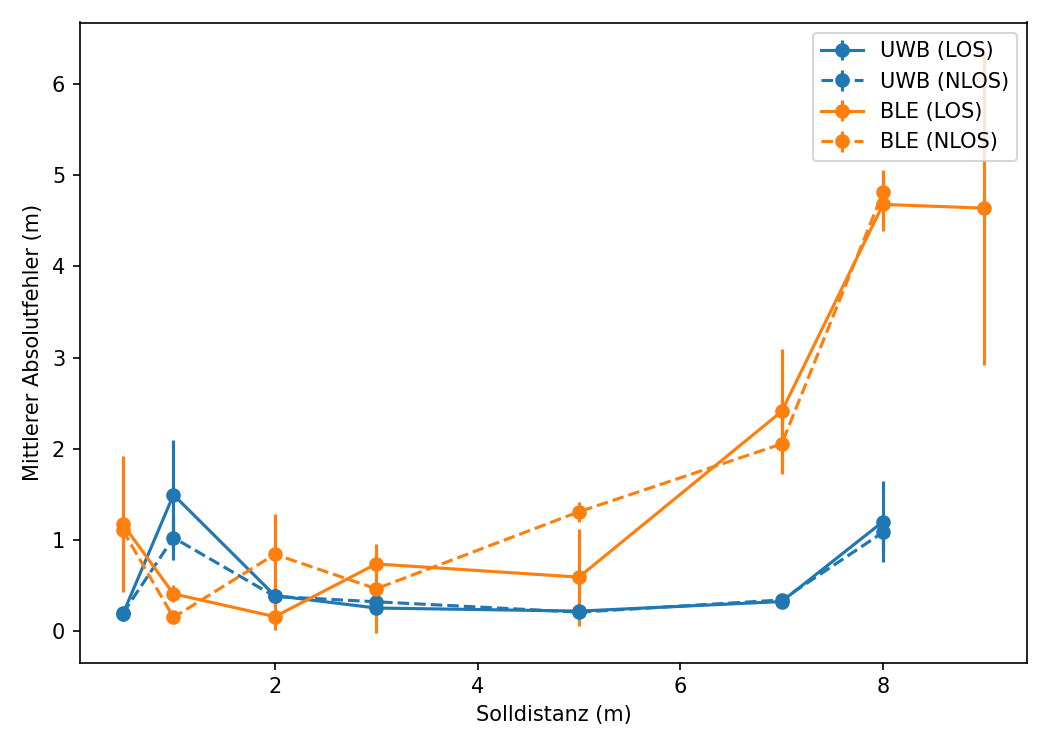
\includegraphics[width=0.7\linewidth]{../abbildungen/m3_uwb_vs_ble.png}
\caption{UWB gegen BLE-RSSI: mittlerer Absolutfehler über die Solldistanz,
LOS durchgezogen, NLOS gestrichelt.}
\label{fig:m3}
\end{figure}

\subsubsection{M4 -- LiDAR-Tiefenmessung gegen Maßband}
\label{sec:m4}

Tabelle~\ref{tab:m4} zeigt den mittleren Absolutfehler aus
\texttt{analysis/evaluation/m4\_lidar.py}, getrennt nach Tag- und
Nachtaufnahme.

\begin{table}[htbp]
\centering
\small
\caption{M4 -- mittlerer Absolutfehler (m) nach Distanz und Tageszeit}
\label{tab:m4}
\begin{tabularx}{\linewidth}{@{}lrr@{}}
\toprule
\textbf{Distanz (m)} & \textbf{MAE nachts (m)} & \textbf{MAE tags (m)} \\
\midrule
0{,}3 & 0{,}0013 & 0{,}0045 \\
0{,}5 & 0{,}0012 & 0{,}0057 \\
1{,}0 & 0{,}0021 & -- \\
2{,}0 & 0{,}0124 & 0{,}0117 \\
3{,}0 & 0{,}0123 & 0{,}0290 \\
4{,}0 & 0{,}0137 & 0{,}0046 \\
5{,}0 & 0{,}0047 & 0{,}0044 \\
17{,}0 & -- & 0{,}5474 \\
\bottomrule
\end{tabularx}
\end{table}

Im spezifizierten Bereich (0,3--5~m) bleibt der Fehler durchweg im
Millimeterbereich, bei Tag wie bei Nacht -- LiDAR ist von den vier
Verfahren das mit Abstand genaueste im Nahbereich. Die 17-m-Messung war
eine bewusste Reichweitentestmessung außerhalb der Scanner-Spezifikation
(rund 5~m) und zeigt entsprechend den erwarteten Fehlersprung auf
0{,}55~m -- ein Beleg der Reichweitengrenze durch Messung statt durch
Behauptung. Die Lücke bei 1~m tagsüber ist eine offene, unkritische
Protokolllücke.

\begin{figure}[htbp]
\centering
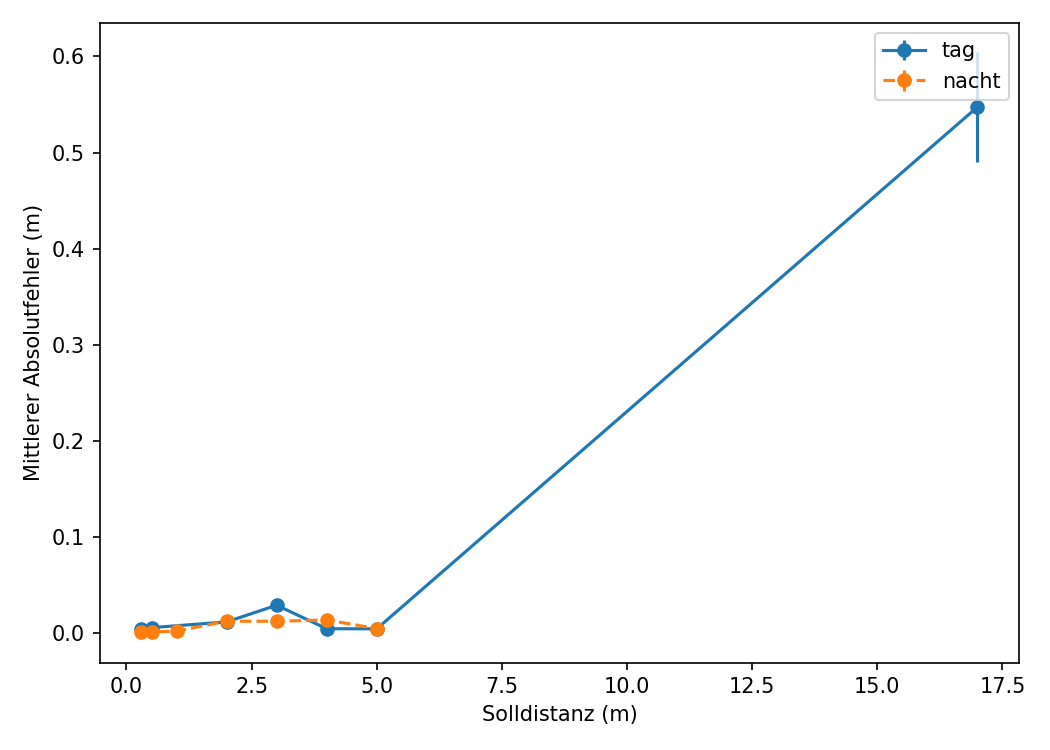
\includegraphics[width=0.7\linewidth]{../abbildungen/m4_lidar.png}
\caption{LiDAR: mittlerer Absolutfehler über die Solldistanz, Tag gegen
Nacht.}
\label{fig:m4}
\end{figure}

\subsubsection{Ortungskaskade: alle vier Verfahren im Vergleich}

Abbildung~\ref{fig:cascade}, erzeugt mit
\texttt{analysis/evaluation/cascade.py}, stellt die drei bisher gemessenen
Verfahren gegenüber: GNSS als globale, distanzunabhängige Referenzlinie bei
der über alle drei Referenzpunkte gewichteten CEP95, UWB und BLE über die
in M3 getestete Distanz, LiDAR über die in M4 getestete Distanz. Das ist
die in
Abschnitt~\ref{sec:messstudien} angekündigte Kaskade -- eine Erweiterung um
den vierten Punkt (M2) bleibt bis zum eigenen Feldtest aus, da
Transportmodus-Klassifikation keine Fehlerangabe in Metern liefert und
nicht in dieselbe Achse passt.

\begin{figure}[htbp]
\centering
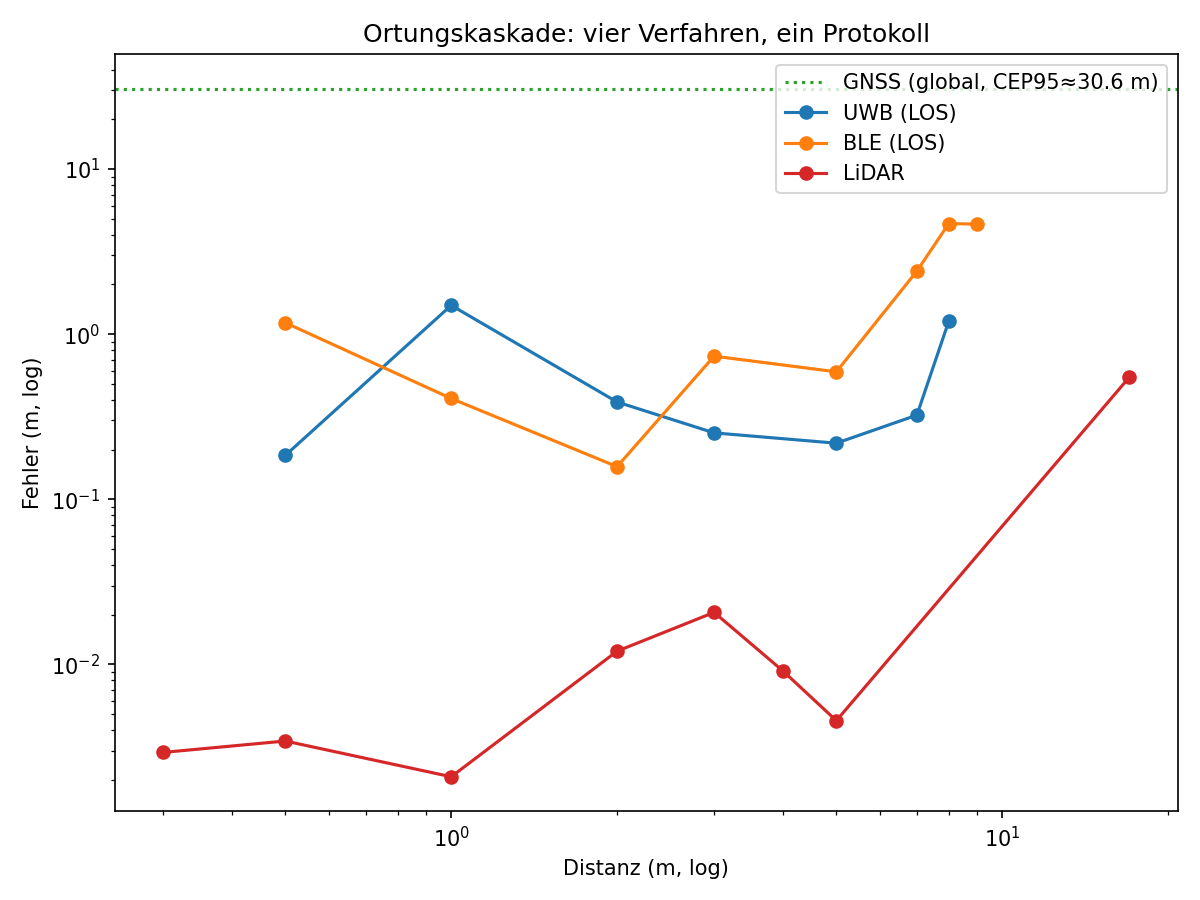
\includegraphics[width=0.85\linewidth]{../abbildungen/cascade.png}
\caption{Ortungskaskade: Fehler über Reichweite, log-log, für GNSS, UWB,
BLE-RSSI und LiDAR.}
\label{fig:cascade}
\end{figure}

\section{Arbeitsteilung}

\begin{description}
    \item[Paul Tschätsch -- Arbeitspaket~1, GeoIoT-Nahbereichsortung]
    UWB-Ranging, Bluetooth-RSSI-Ranging, LiDAR-Tiefenmessung und deren
    Auswertung (M3, M4).
    \item[Carl Janek Markert -- Arbeitspaket~2, Klassifikation und GeoAI]
    Transportmodus-Klassifikation, Segmentierung und deren Auswertung
    (M1, M2).
\end{description}

Die eingefrorene Schnittstelle zwischen beiden Paketen ist die
\texttt{Segment}-Tabelle: Arbeitspaket~2 erzeugt \texttt{predicted\_mode}
und \texttt{label\_mode} je Segment, Arbeitspaket~1 liest \texttt{start\_ts}
und \texttt{end\_ts} für die Zuordnung der GeoIoT-Messungen zu denselben
Zeiträumen, ohne die Klassifikationslogik selbst anzufassen.

\section{Diskussion}

\subsection{Grenzen}

\begin{enumerate}
    \item \textbf{Klasse \emph{plane} strukturell unterrepräsentiert.} Von
    56 GeoLife-Nutzern haben vier Flugdaten aufgezeichnet, insgesamt
    9174~von 5,45~Mio. Fixes (0{,}17~Prozent). Das trainierte Modell
    erreicht für diese Klasse ein F1 von 0{,}019 (Precision~1{,}0,
    Recall~0{,}009 bei 107~Testbeispielen) -- kein Trainingsfehler, sondern
    eine Grenze des verfügbaren Datensatzes. Gegenmaßnahme: Das
    Abgabedokument weist \texttt{macro\_f1\_ohne\_plane} zusätzlich zum
    regulären Macro-F1 aus.
    \item \textbf{Klassen \emph{foot} und \emph{bike} bei kleiner
    Trainingsstichprobe kaum trennbar.} Ein Trainingslauf auf 20 von 56
    Nutzern erreichte für \emph{bike} ein F1 zwischen 0{,}11 und 0{,}17;
    derselbe Lauf auf allen 56~Nutzern erreichte 0{,}670. Gegenmaßnahme:
    Der volle Datensatz ist Standard in \texttt{geolife/train.py}, die
    Stichprobenfunktion bleibt nur für schnelle Entwicklungsläufe erhalten.
    \item \textbf{M2 (Klassifikationsgüte im Feldtest) bislang nur n=6.}
    Sechs reale Segmente aus vier Aufzeichnungen liegen vor
    (Abschnitt~\ref{sec:m2}); der geplante Mehrmodi-Feldtest mit mehreren
    Verkehrsmitteln, längeren Segmenten und Stopps fehlt noch -- die in
    Abschnitt~\ref{sec:befund-training} genannte Modellgüte
    (Macro-F1~0{,}704) stammt weiterhin aus dem GeoLife-Testsplit, nicht aus
    eigenen Trips. Auf den sechs vorliegenden Segmenten liegt das eigene
    Modell leicht unter der Systembaseline (Macro-F1 0{,}54 gegen 0{,}62) bei
    gleicher Trefferquote (je vier von sechs); es gewinnt bei \emph{train}
    und verliert bei \emph{bike}, beide Klassen mit höchstens zwei
    Segmenten belegt. Diese Arbeit behauptet an
    keiner Stelle, das Modell funktioniere auf selbst aufgezeichneten Daten
    ebenso gut wie auf dem Testsplit.
    \item \textbf{M3/M4-Reichweitengrenzen unterhalb der Spezifikation.}
    UWB-Ranging brach bei 9~m zuverlässig ab (Abschnitt~\ref{sec:m3}),
    LiDAR zeigt bei 17~m einen deutlichen Fehlersprung
    (Abschnitt~\ref{sec:m4}). Beide Verfahren sind für den in dieser App
    vorgesehenen Nahbereich (unter 5~m) unkritisch, für größere Distanzen
    aber nicht geeignet.
\end{enumerate}

\subsection{Abweichungen von der Projektskizze}
\label{sec:abweichungen}

Die Projektskizze vom 02.06.2026 war als Orientierung gedacht und ist
durch die Einreichung änderbar. Tabelle~\ref{tab:abweichungen} führt auf,
wo die Umsetzung von ihr abweicht; die beiden größten Änderungen -- Ortung
als Messgegenstand statt als Voraussetzung, und der Verzicht auf die
Fahrtbericht-Generierung -- sind in
Abschnitt~\ref{sec:leitmotiv} und \ref{sec:gestrichen} begründet.

\begin{table}[htbp]
\centering
\small
\caption{Projektskizze gegen Umsetzung}
\label{tab:abweichungen}
\begin{tabularx}{\linewidth}{@{}>{\raggedright\arraybackslash}p{3.1cm}>{\raggedright\arraybackslash}p{4.2cm}L@{}}
\toprule
\textbf{Skizze} & \textbf{Umsetzung} & \textbf{Anmerkung} \\
\midrule
GNSS L1/L5, dGPS über NTRIP, dezimetergenau &
\texttt{CoreLocation}-GNSS, Genauigkeit gemessen (M1) &
kein NTRIP; die Genauigkeit wird belegt statt vorausgesetzt \\
\addlinespace
UWB und BLE &
UWB und BLE-RSSI gegen Maßband (M3) &
umgesetzt \\
\addlinespace
Transportmodus per ML (TensorFlow Lite) &
Random Forest (\texttt{scikit-learn}), Export nach Core~ML &
Abschnitt~\ref{sec:entwurf-modell} \\
\addlinespace
React Native oder Flutter, iOS und Android &
natives SwiftUI, nur iOS &
UWB, LiDAR und BLE-Ranging liegen in iOS-Frameworks
(\texttt{NearbyInteraction}, \texttt{ARKit}, \texttt{CoreBluetooth}) \\
\addlinespace
SQLite, PostGIS-kompatibel &
SQLite über GRDB, Export als CSV und GeoJSON &
kein PostGIS; die Auswertung läuft in Python auf den Exporten \\
\addlinespace
LLM-Reisetagebuch &
gestrichen &
Abschnitt~\ref{sec:gestrichen} \\
\addlinespace
Fotos georeferenziert organisieren &
nicht umgesetzt &
nicht Teil der Messkette \\
\addlinespace
Karte mit Routen, Heatmaps, Zeitraffer-Replay &
MapLibre-Karte in der App, Replay im Standalone-Viewer &
keine Heatmaps \\
\bottomrule
\end{tabularx}
\end{table}

\subsection{Gestrichen: die Fahrtbericht-Generierung}
\label{sec:gestrichen}

Die Projektskizze sah als zweiten Anwendungsfall vor, aus einem
abgeschlossenen Trip über ein Sprachmodell einen Fahrtbericht zu erzeugen
und diese Texte anschließend auf Halluzinationen zu prüfen. Beides war
implementiert: ein Client gegen die Gemini-API in der App, dazu ein
Prüfskript, das jeden erzeugten Text gegen das Trip-JSON hält und ungedeckte
Orte, Verkehrsmittel, Zahlen und Ereignisse meldet.

Gestrichen wurde der Teil dennoch, aus einem Grund, der sich erst über die
Messstudien ergab: Was hier entstanden ist, ist eine Messanwendung, keine
Reise-App. Die vier Ortungsverfahren und ihre gemeinsame Prüfkette tragen
die Arbeit (Abschnitt~\ref{sec:leitmotiv}); die Transportmodus-Klassifikation
gehört dazu, weil sie dieselbe Frage auf einer anderen Ebene stellt und mit
M2 dieselbe Art von Sollwertvergleich bekommt. Ein erzeugter Fließtext hat
diese Eigenschaft nicht. Er lässt sich gegen seine Eingabedaten prüfen, aber
er misst nichts, und er hätte als einziger Bestandteil der Arbeit keinen
Platz in der Kaskadenabbildung gefunden -- Halluzinationsrate ist kein
Fehler in Metern über einer Reichweite.

Die Alternative wäre gewesen, den Teil mitzuschleppen und im Diskussionsteil
als ungeprüft auszuweisen. Eine Komponente ohne Messergebnis schwächt eine
Arbeit, deren Kernaussage lautet, dass jedes Verfahren seine eigene
Prüfkette braucht. Der Schnitt ist deshalb der ehrlichere Weg als ein
sechster Punkt auf der Aufgabenliste, zu dem keine Zahl vorliegt.

\subsection{Umsetzungsstand}

\begin{table}[htbp]
\centering
\small
\caption{Was vorliegt und was aussteht}
\label{tab:stand}
\begin{tabularx}{\linewidth}{@{}>{\raggedright\arraybackslash}p{4.2cm}L@{}}
\toprule
\textbf{Stand} & \textbf{Inhalt} \\
\midrule
umgesetzt und geprüft & Aufzeichnung, Segmentierung, Transportmodus-Klassifikation,
UWB-/BLE-/LiDAR-Messwerkzeuge mit CSV-Export,
67 automatisierte Tests \\
\addlinespace
durch Prüflauf belegt & Macro-F1 0{,}704 ohne \emph{plane} auf dem
vollständigen GeoLife-Datensatz; Modellgröße 27~statt 802~Megabyte; M1
(GNSS, alle drei Referenzpunkte, Tabelle~\ref{tab:m1}); M3 (UWB/BLE,
Tabelle~\ref{tab:m3}); M4 (LiDAR, Tabelle~\ref{tab:m4}); M2 (sechs reale
Segmente, Tabelle~\ref{tab:m2}); Ortungskaskade (Abbildung~\ref{fig:cascade});
Viewer; \texttt{run\_all.py} \\
\addlinespace
nicht Teil dieser Abgabe & M2 vollständiger Mehrmodi-Feldtest
(Abschnitt~\ref{sec:m2}) \\
\addlinespace
im Verlauf gestrichen & Fahrtbericht-Generierung über ein Sprachmodell
(Abschnitt~\ref{sec:gestrichen}) \\
\bottomrule
\end{tabularx}
\end{table}

Was diese Abgabe ausdrücklich \emph{nicht} behauptet: eine belegte Aussage
über die Trefferquote des Klassifikationsmodells auf selbst aufgezeichneten
Trips im Allgemeinen -- n=6 trägt keine Verallgemeinerung. Für M1, M3
und M4 liegen belastbare Felddaten vor, für M2 sechs erste echte, aber
wenige Datenpunkte, auf denen das eigene Modell schlechter abschneidet als
die Systembaseline, siehe Abschnitt~\ref{sec:messstudien}.

\section{Fazit}

Der Wechsel von Gradient Boosting zu Random Forest war keine reine
Geschwindigkeitsentscheidung: Erst die Kontrolle über die Baumtiefe machte
den Unterschied zwischen einem 802~Megabyte großen und einem
27~Megabyte großen Modell aus, bei identischer Genauigkeit. Der
Befund aus Abschnitt~\ref{sec:befund-training} zeigt denselben Punkt aus
einer anderen Richtung: Eine Modellschnittstelle, die aus einem Plan statt
aus dem tatsächlich exportierten Artefakt abgeleitet wird, trägt Annahmen,
die erst am erzeugten Code sichtbar werden.

Die eigene Messreihe (Abschnitt~\ref{sec:messstudien}) bestätigt die aus
der Literatur erwartete Rangfolge: UWB liegt bei fünf von sieben
Solldistanzen unter 0{,}4~m MAE und misst dabei sehr reproduzierbar, mit
konstanter Verzerrung nach oben; die Ausnahmen sind 1~m (ein ungeklärter
Versatz um etwa 1~m) und 8~m (Reichweitengrenze). BLE-RSSI degradiert ab
5~m deutlich und erreicht bei 8--9~m einen MAE von fast 5~m.

Bei M2 fällt das Ergebnis gegen die eigene Erwartung aus, und der Grund
dafür ist selbst ein Befund (Abschnitt~\ref{sec:befund-segmenter}): Eine
defekte Stopperkennung, die auf Realdaten praktisch nie feuerte, blieb
durch drei Segmenter-Tests mit exakt regelmäßigen synthetischen
Zeitstempeln unentdeckt, bis der Feldtest vom 20.09. eine 56-minütige
Aufzeichnung als ein einziges durchgehendes Segment zeigte. Nach der
Korrektur kippt ein zuvor dokumentierter Treffer -- das Modell hatte eine
Zugfahrt korrekt als \emph{train} erkannt -- zu \emph{car}, weil sich mit
der Fenstergrenze auch die Merkmale ändern, die der Klassifikator sieht.

Die Kernthese dieser Arbeit (Abschnitt~\ref{sec:leitmotiv}) besteht aus
zwei Teilen, und die sechs Segmente trennen sie. Der strukturelle Teil
hält: \texttt{CMMotionActivity} meldete auf beiden Zugfahrten überwiegend
\texttt{automotive} und kann \emph{train} nicht vergeben, weil die Klasse in
seinen fünf Zuständen nicht existiert; das eigene Modell trifft eine der
beiden Fahrten. Der empirische Teil hält nicht: Bei gleicher Trefferquote
(je vier von sechs) liegt das eigene Modell mit einem Macro-F1 von 0{,}54
knapp unter der Systembaseline mit 0{,}62, weil es die Radfahrt verfehlt,
die die Baseline trifft. Ein Modell, das eine Klasse abbilden kann, die die
Systemschnittstelle nicht kennt, ist damit kein Modell, das im Feld
insgesamt besser klassifiziert -- auf diesen Daten tauscht es eine Schwäche
gegen eine andere.

Das ist bei sechs Segmenten aus vier Klassen kein Gegenbeweis, sondern ein
offener Punkt mit einem klaren Prüfverfahren: derselbe Vergleich über
mindestens drei Segmente je Klasse. Solange der nicht gefahren ist, steht
die Verallgemeinerung der GeoLife-Güte (Macro-F1~0{,}704) auf eigene Trips
ohne Beleg da -- und diese Arbeit behauptet sie deshalb nicht.

\section{Verwendete Hilfsmittel}

Werkzeuge: Xcode 26, xcodegen, GRDB~7, MapLibre~6.29, coremltools~8.1,
scikit-learn~1.5.2, pandas, matplotlib, pyproj, tectonic~0.16.9.

Regel im Umgang mit KI-Vorschlägen: Codevorschläge, die eine von
\texttt{coremltools} oder Xcode automatisch erzeugte Schnittstelle
voraussetzen, werden gegen die tatsächlich generierte Schnittstelle
geprüft (\texttt{xcrun coremlcompiler generate} beziehungsweise ein
direkter Testaufruf), nicht gegen die Dokumentation oder den
Implementierungsplan allein übernommen. Anlass war der Befund aus
Abschnitt~\ref{sec:befund-training}: Ein aus dem Plan übernommenes
Codebeispiel benannte ein Ausgabefeld, das im tatsächlichen Modell nicht
existiert.

\section*{Lizenzen und Attribution}
\addcontentsline{toc}{section}{Lizenzen und Attribution}

GeoLife GPS Trajectories (Microsoft Research Asia) -- Nutzung für
nicht-kommerzielle Forschungszwecke gemäß den Nutzungsbedingungen des
Datensatzes. ALKIS Berlin Gebäude (Land Berlin, WFS-Dienst) -- Datenlizenz
Deutschland, Namensnennung~2.0. Nominatim/OpenStreetMap-Geokodierung für
die Referenzpunkte~p2 und~p3 -- Open Database License, Attribution
\textcopyright{} OpenStreetMap-Mitwirkende. MapLibre GL Native -- BSD-2-Clause.
GRDB.swift -- MIT-Lizenz. Bei unterschiedlichen Lizenzbedingungen der
genannten Quellen gilt die jeweils restriktivere Bedingung für den
gesamten Datensatzabschnitt, der aus ihr abgeleitet ist.

\begin{thebibliography}{9}
\bibitem{geolife}
ZHENG, Yu; XIE, Xing; MA, Wei-Ying (2010).
\textit{GeoLife: A Collaborative Social Networking Service among User,
Location and Trajectory}. IEEE Data Engineering Bulletin, 33(2), 32--40.

\bibitem{ieee802154z}
IEEE (2020).
\textit{IEEE Std 802.15.4z-2020 -- Enhanced Ultra-Wideband (UWB) Physical
Layers (PHYs) and Associated Ranging Techniques}. IEEE Standards
Association.

\bibitem{wgs84}
NATIONAL GEOSPATIAL-INTELLIGENCE AGENCY (2014).
\textit{World Geodetic System 1984 (WGS84)}, NGA.STND.0036\_1.0.0\_WGS84.
\end{thebibliography}

\end{document}
